\subsection{Explicación del algoritmo y Complejidad.}

\vspace*{0.3cm}

Tenemos dos vecindades posibles, la primera es, dado un grafo, voy a ir recorriendo nodo a nodo, buscando si posee, algún color que nos beneficie
en la cantidad de conflictos totales. En el caso de encontrarlo, cortara el seguimiento, y se volverá a llamar recursivamente, hasta no encontrar
algún color que genere menos conflictos totales. Si ningún nodo contiene algún color que genere menor cantidad de conflictos totales, entonces 
el programa termina, llegando a un mínimo local.
La segunda vecindad,considerar solo modificaciones en los nodos con mayor cantidad de conflictos, ya que es mas probable que al cambiarles el color, puedan
llegar a mejorar bastante la cantidad de conflictos generados. Y luego intentara buscar algún color que nos beneficie, buscando sobre los nodos
que generan mas conflictos.

Pero antes de llamar al algoritmo de cada una de estas vecindades, agarramos el grafo inicial que nos dan, en el cual viene cada nodo con sus sucesores y con sus colores posibles, y asignamos a cada nodo un color random sobre los que tiene, y luego llamaremos a la función de heuristicaLocal, para alguna de las dos vecindades. La función que utilizamos para obtener un mínimo local, es decir la función que utilizamos para medir la calidad de una solución, es cuantos conflictos genera la misma.

\textbf{ Nota:} Son vecindades distintas ya que una esta contenida en la otra. Una vecindad(heurística 1) considera como vecinas de una solución a todas las posibles modificaciones de un color en cualquier nodo. La otra vecindad esta contenida en la anterior, ya que considera como vecinos a las posibles modificaciones de un color, pero  \textbf{\underline{solo}} en los nodos que tienen un máximo de cantidad de conflictos.

PseudoCódigo Heurística 2:


\begin{codebox}
\Procname{$\proc{hueristica2}(Nodo[] \ grafo)$}
	\li	Nodo[] $nodosMayorCantidadConflictos$ = buscoLosNodosQueMasConflictosGeneran($grafo$) 
	\li 	// -> nodosConflictos, son los todos los nodos que tienen la mayor cantidad
	\li 	//  de conflictos,y luego iterare por estos, en busqueda de una cantidad 
	\li 		//  menor de conflictos totales.
	\li 		//  La complejidad de este ordenamiento es n cuadrado, esta explicado mejor en el codigo
	\li	for Nodo $nodoActual$ in $nodosMayorCantidadConflictos$ do 
	\li 		//Esto se hace como mucho n veces * O(c*n*n)
	\li		for int $color$ in $nodoActual$.getColoresPosibles() do  
	\li 			// Esto se hace como mucho, cantColores(c) veces * O(n) = O(c*n)
	\li			$conflictosDiferencia$ = calcularCantidadConflictos($nodosGrafo$, $i$, $color$) // O(n) 
	\li			\If mayor($conflictosDiferencia$, $0$)
	\li 				//Entonces, el color "nuevo" genera menos conflictos, entonces debo cambiarlo!!
	\li				\Then	$conflictosInicial$ = $conflictosInicial$ - $conflictosDiferencia$ // Le saco la diferencia de conflictos, que tenia el anterior
	\li 						// color, con el nuevo!! Es la forma de actualizar la cantidad de conflictos totales, sin tener que volver a calcularlo.
	\li						$huboMejora$ = $true$
	\li						$nodosGrafo[i]$.setColor($color$) // O(1)
				\End
	\li 		end for
	\li		\If huboMejora do
	\li			\Then	break busqueda
			\End
	\li 		end for
	\li	\If $huboMejora$  // O(1)
	\li		\Then	mejorarSiPosible2($nodosGrafo$, $conflictosInicial$) //Me llamo recursivamente!! 
		\End
\end{codebox}

Un paso a paso mas detallado seria: primero vamos a recorrer nodo a nodo(linea 6), fijándonos si contiene algún color que reduzca la cantidad
de conflictos(linea 10) si lo encontramos, entonces nos guardamos la cantidad de conflictos que generan, avisamos que hubo una mejora(linea 15)
y luego cortamos la circulación del programa para lanzarlo de nuevo, así buscamos nuevamente los nodos que mas conflictos generan.(linea 19)


La función calcularCantidadConflictos(pseudo):

\begin{codebox}
\Procname{$\proc{calcularCantidadConflictos}(Nodo[] \ nodosgrafo, int \ i, int \ color)$}
	\li int $cantConflictosOriginal, cantConflictosColor$ = $0$ //O(1)
	\li 	\For $sucesor$ in  $nodosGrafo[i]$.getSucesores() \do  // se corre n veces como mucho, => O(n)* O(1) => O(n)
	\li 		\If $sucesor$.tieneColor() y $sucesor$.getColor() == $nodosGrafo[i]$.getColor() do // O(1)
	\li 			\Then	$cantConflictosOriginal++$ //O(1)
	 		\End
	\li  	\If $sucesor$.tieneColor() y $sucesor$.getColor() == $color$ //O(1)
	\li 			\Then	$cantConflictosColor++$  //O(1)
			\End
	\li	end for
	\li	return $cantConflictosOriginal$ - $cantConflictosColor$;	// Si esto es positivo, quiere decir que el color "nuevo" tiene menos conflictos
	\li 		// Entonces, vamos a devolver esta diferencia, y vamos a cambiar el color.
	\li 		// La complejidad del algoritmo es O(n)
\end{codebox}

Para una explicación mas detallada de las complejidades, ver el apéndice con el código. El resultado obtenido para ambas es de $ c*m*n^2 $.


\subsection{Experimentación y gráficos.}

\vspace*{0.3cm}

\subsubsection{Test 1}

\vspace*{0.3cm}

\begin{figure}[H]
  \begin{center}
      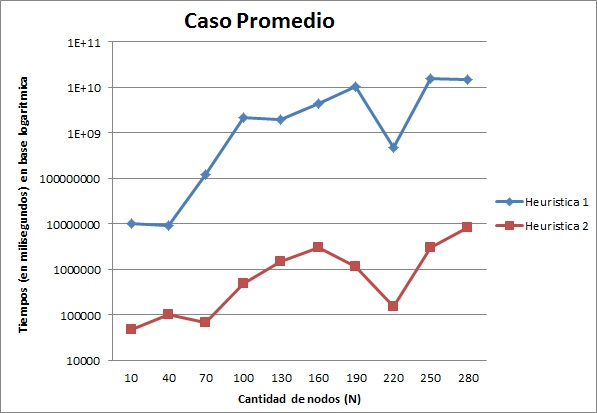
\includegraphics[scale=0.75]{../Ejercicio4Promedio.jpg}
  \end{center}
  \caption{Tiempos caso promedio, comparando las dos heurísticas locales sobre los mismos grafos}
\end{figure}

\begin{figure}[H]
  \begin{center}
      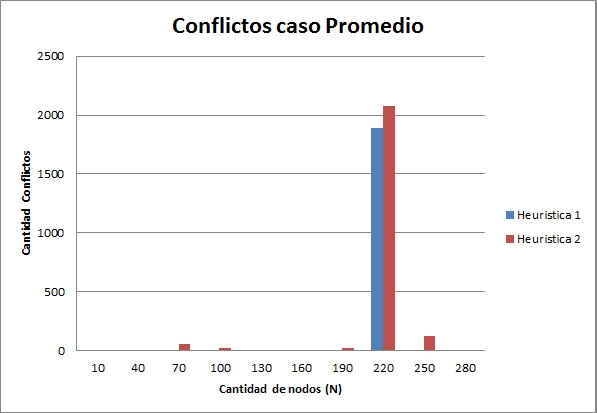
\includegraphics[scale=0.75]{../Ejercicio4PromedioConflictos.jpg}
  \end{center}
  \caption{Conflictos caso promedio, comparando las dos heurísticas locales sobre los mismos grafos}
\end{figure}

En este gráfico (caso promedio), se puede ver bien que la heurística numero 1 , es mas lenta que la segunda, pero sin embargo viendo el gráfico de caso promedio conflictos, se puede ver que es mejor, ya que tiene una menor cantidad de conflictos.

\subsubsection{Test 2}

\vspace*{0.3cm}

\begin{figure}[H]
  \begin{center}
      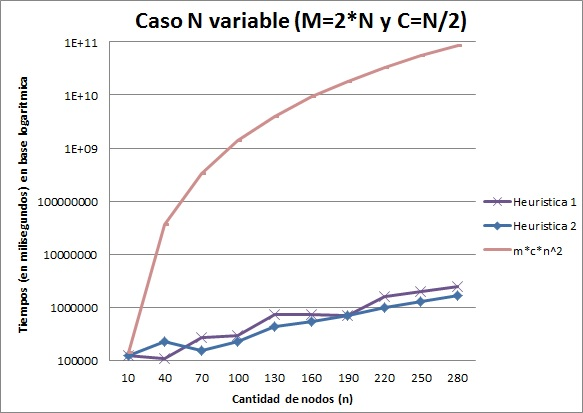
\includegraphics[scale=0.75]{../Ejercicio4NVariable.jpg}
  \end{center}
  \caption{Tiempos caso N variable, manteniendo la multiplicación de M y C constantes}
\end{figure}

El gráfico de N variable, muestra que el tiempo que tarda en correr el algoritmo de ambas heurísticas esta acotado por la complejidad que es $m*n^2*c$, y que ambas tardan tiempos parecidos, pero suponemos que es porque al hacer crecer n, y mantener a $m = 2n$ y $c=n/2$ (de esta manera la multiplicación conserva su valor) la cantidad de colores es constante, pero m termina siendo bastante chica de lo que podría ser, haciendo que el grafo tenga pocas aristas comparado con las que podría tener, que son $n*(n-1)/2$.

\subsubsection{Test 3}

\vspace*{0.3cm}

\begin{figure}[H]
  \begin{center}
      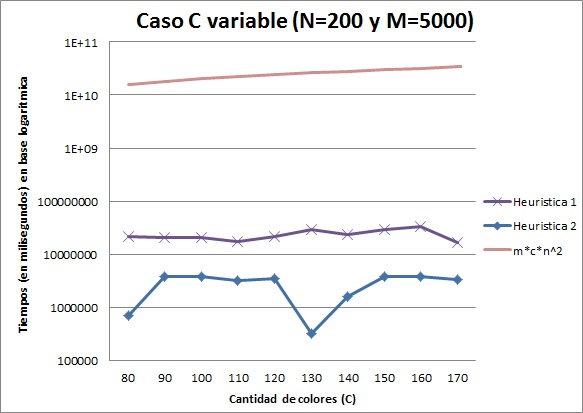
\includegraphics[scale=0.75]{../Ejercicio4CVariable.jpg}
  \end{center}
  \caption{Tiempos caso C variable, manteniendo fijos los valores de M y N}
\end{figure}
  
\begin{figure}[H]
  \begin{center}
      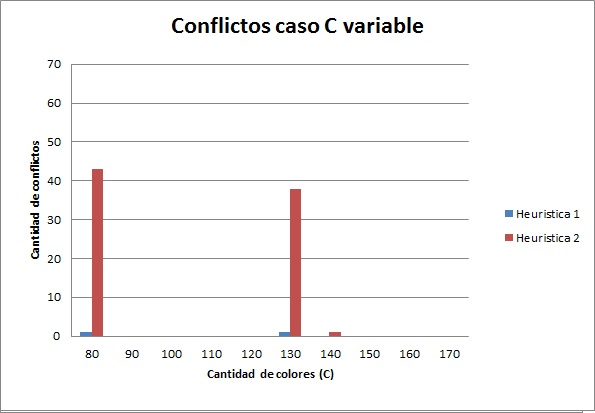
\includegraphics[scale=0.75]{../Ejercicio4CVariableConflictos.jpg}
  \end{center}
  \caption{Conflictos caso C variable, manteniendo fijos los valores de M y N}
\end{figure}

Grafo c variable, muestra que esta acotado por la complejidad de $m*n^2*c$, y vuelve a mostrar que la heurística 1, es mas lenta que la heurística 2. Y el gráfico de conflictos de c, sigue corroborando, que la heurística 2 se estanca en un mínimo local mas grande, generando mas conflictos.

\subsubsection{Test 4}


\begin{figure}[H]
  \begin{center}
      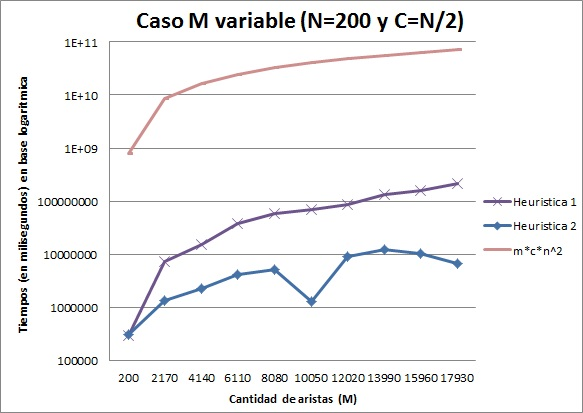
\includegraphics[scale=0.75]{../Ejercicio4MVariable.jpg}
  \end{center}
  \caption{Tiempos caso M variable, manteniendo fijos los valores de N y C}
\end{figure}

\begin{figure}[H]
  \begin{center}
      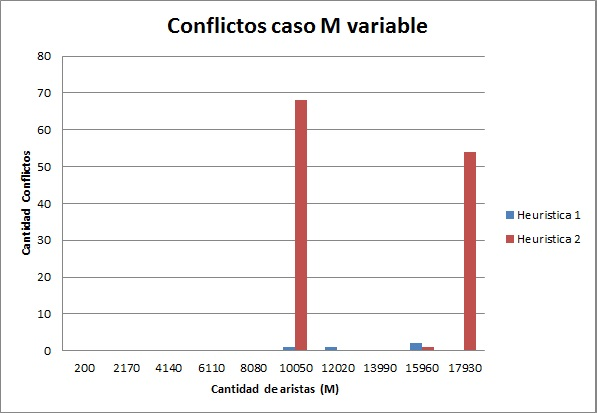
\includegraphics[scale=0.75]{../Ejercicio4MVariableConflictos.jpg}
  \end{center}
  \caption{Conflictos caso M variable, manteniendo fijos los valores de N y C }
\end{figure}

En el gráfico de m variable, del ejercicio 4, se puede ver claramente que la segunda heurística es mas rápida, pero que generalmente, tiene una cantidad de conflictos mas grande. Se puede ver en el gráfico de m variable conflictos, a lo que suponemos que es porque al resolver por mayor cantidad de conflictos que genera un nodo, al cambiarle el color es mas probable que haya una menor cantidad de conflictos. Y al cambiarlo e ir arreglando de a muchos conflictos, corre menos iteraciones del algoritmo, pero se estanca en un mínimo local mas grande.
